The Large Hadron Collider (LHC) is the largest 
particle accelerator and collider in the world.
The LHC is built in a circular tunnel 27 km in circumference 
that is buried between 50 m to 175 m underground 
and straddles the Swiss and the French borders 
at CERN.
The LHC is a synchrotron that accelerates two counter-rotating beams of
protons  to 6.5 \TeV~then brings them into head-on collisions at the center of 
four large detectors: ALICE, ATLAS, CMS, and LHCb. The center of mass energy of the proton-proton (or $pp$)\
collision is $\sqrt{s}=$13 \TeV, the energy of the collision data analyzed in this dissertation.
The beam itself has a total energy of 336 MJ requiring an accurate and careful steering 
of the beam at all times.
This is achieved by a strong magnetic field, generated by 
superconducting magnets, that guides the protons around the accelerator.
There are 1232 dipoles magnets, each 15 meters long operating at 1.9 K and generating a magnetic field of 8.33 T.
The dipoles are comprised of 7600 km of superconducting cable which is formed from filaments of Niobium-titanium (NbTi).
%-- the total length of the filaments is more than 10 AU.

A complex of smaller accelerators boost the protons before
injecting them to the LHC, the last accelerator in the chain as shown in 
Figure~\ref{fig:exp.lhc.CCC}.
\begin{figure}[!htb]
\centering
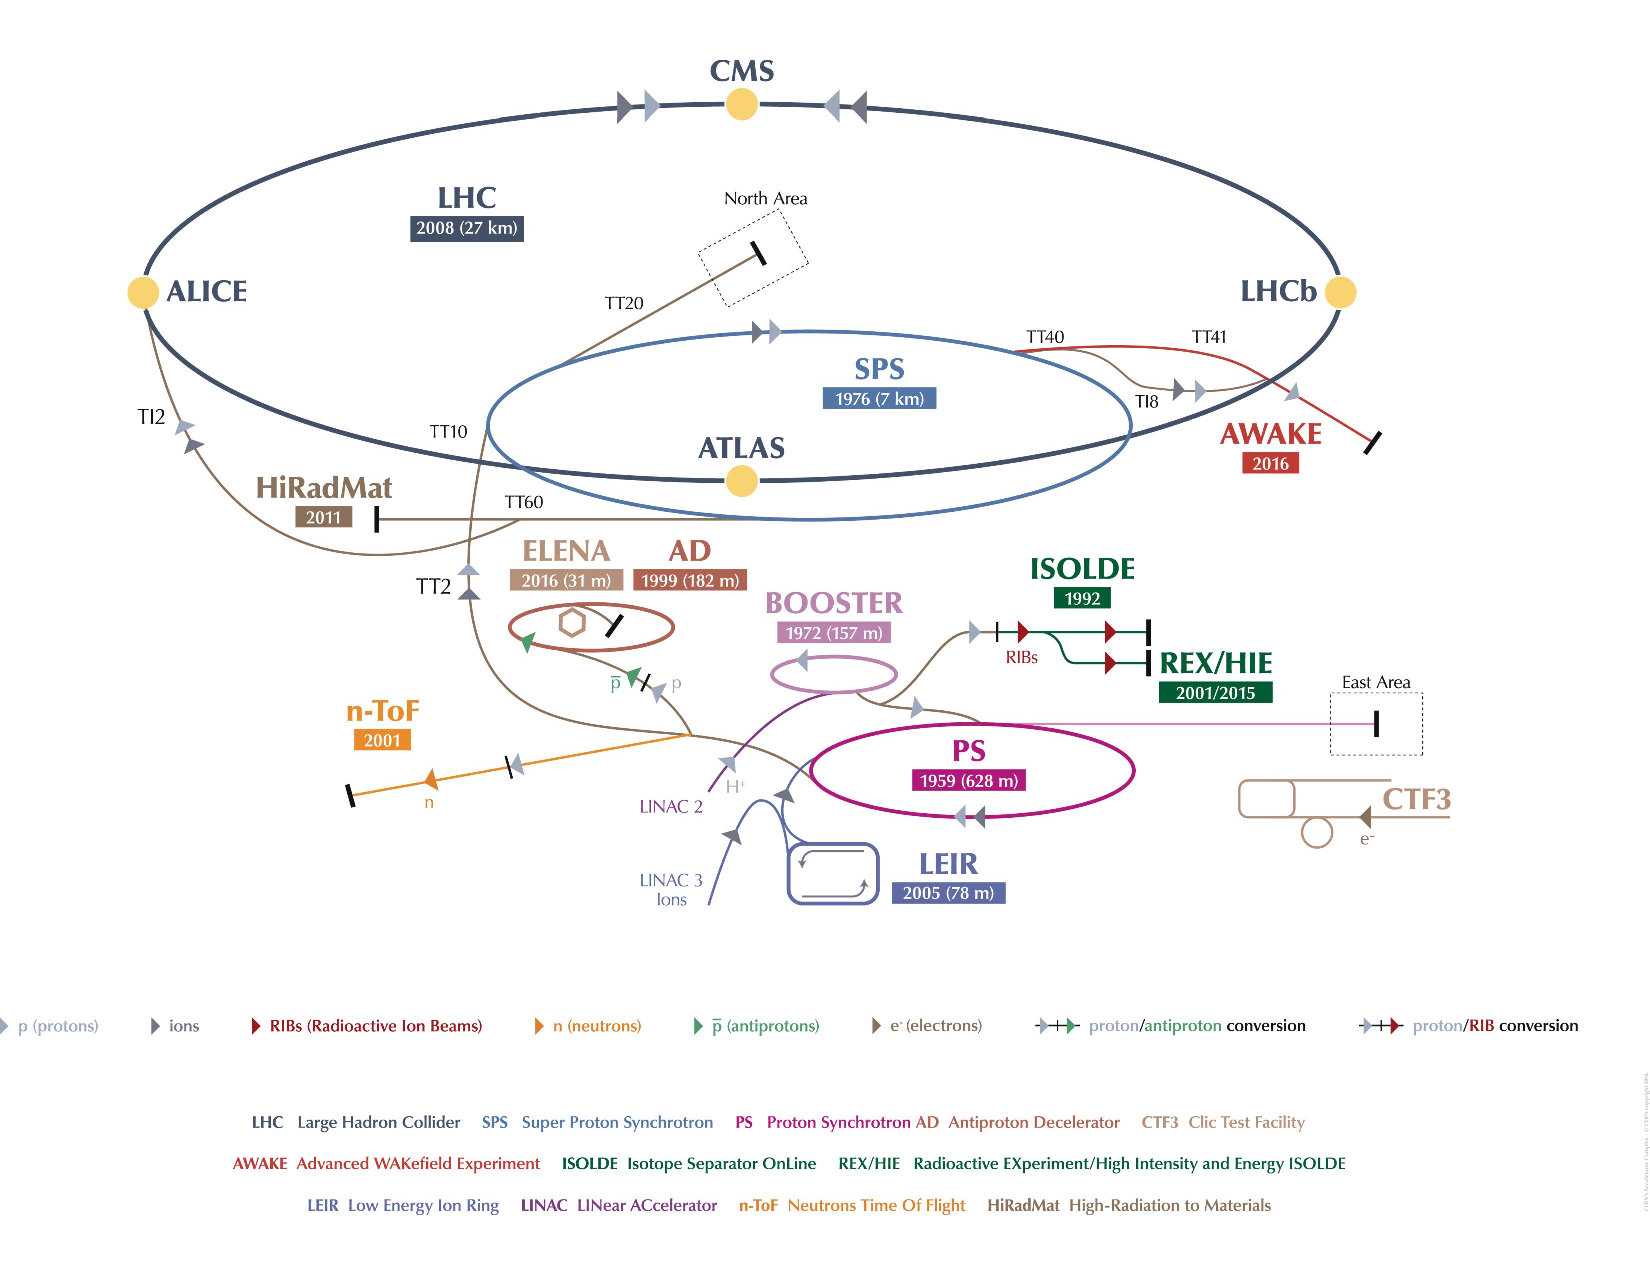
\includegraphics[width=1.\textwidth]{CCC-v2016}
\caption{The CERN accelerator complex 
composed of a chain of  particle accelerators with
the LHC as the last ring (dark blue line) \cite{DeMelis:2197559}.
}
\label{fig:exp.lhc.CCC}
\end{figure} 
Protons, obtained from hydrogen atoms, start their journey in a linear 
accelerator
called the Linac2. The Linac2 accelerates the protons to 50 \MeV. Then, they are injected into
the PS Booster, which accelerates them to 1.4 \GeV. After the PS Booster, the protons are sent to
the Proton Synchrotron (PS) where they are accelerated to 25 GeV. They are then sent to the Super
Proton Synchrotron (SPS) where they are accelerated to 450 \GeV. 
At this stage, the protons are injected into the LHC and accelerated to the target 
energy of 6.5 \TeV~per proton.
 The beams are then focused at each of the interaction points to produce proton-proton collisions.
Under normal operating conditions, the colliding beams will circulate for $\mathcal{O}\left(10\right)$ hours at a time.

The protons are grouped in ``bunches'' when circulated in the LHC as a result of the acceleration 
scheme.
In normal operation of the LHC, each proton beam has 2808 bunches, with each bunch containing 
about 100 billion protons. 
These bunches are a few centimetres long and a few millimeters wide when they are far from a 
collision point but squeezed to about 16 micrometers when they collide.
The rate of their interaction is defined in terms of the luminosity, a 
measure of the number of collisions produced per second by the accelerator.
Generally, the event rate $\frac{dN}{dt}$ of a physics process with cross section $\sigma$ is
\begin{equation}
\frac{dN}{dt} = \sigma  \mathcal{L} 
\label{eq:exp.lhc.lumi}
\end{equation}
where the constant of proportionality, $\mathcal{L}$, is called the instantaneous luminosity,
and has units of $\textrm{cm}^{-2}\textrm{s}^{-1}$.
%\[
% \mathcal{L}  = \frac{n_b N_L N_R f_\text{rev}}{A^\text{eff}_T}
%\]
The LHC has exceeded its design luminosity of $10^{34}\textrm{cm}^{-2}\textrm{s}^{-1}$ or 10 $\textrm{nb}^{-1}\textrm{s}^{-1}$ 
(1 barn = $10^{-24} \textrm{cm}^2$) 
by almost 40\% as shown in Figure~\ref{fig:exp.lhc.peakLumiByFill}.
Given the total inelastic cross section of 60 mb, 
the collision rate of protons is then $ \sigma  \mathcal{L} \sim 10^9$ Hz: a billion proton
interactions per second.
The integral of the instantaneous luminosity, $L = \int  \mathcal{L} dt$, refers to the amount 
of data collected. 
The large integrated luminosities allow for the study of rare processes, such as the search for 
supersymmetric particles.
Figure~\ref{fig:exp.lhc.intlumivsyear} shows the data sets collected by the LHC,
 where the data collected in 2015 and 2016 at $\sqrt{s}=13$ \TeV~is the basis of the work 
presented in this dissertation. 

\begin{figure}[!htb]
\centering
\begin{subfigure}[t]{0.48\textwidth}
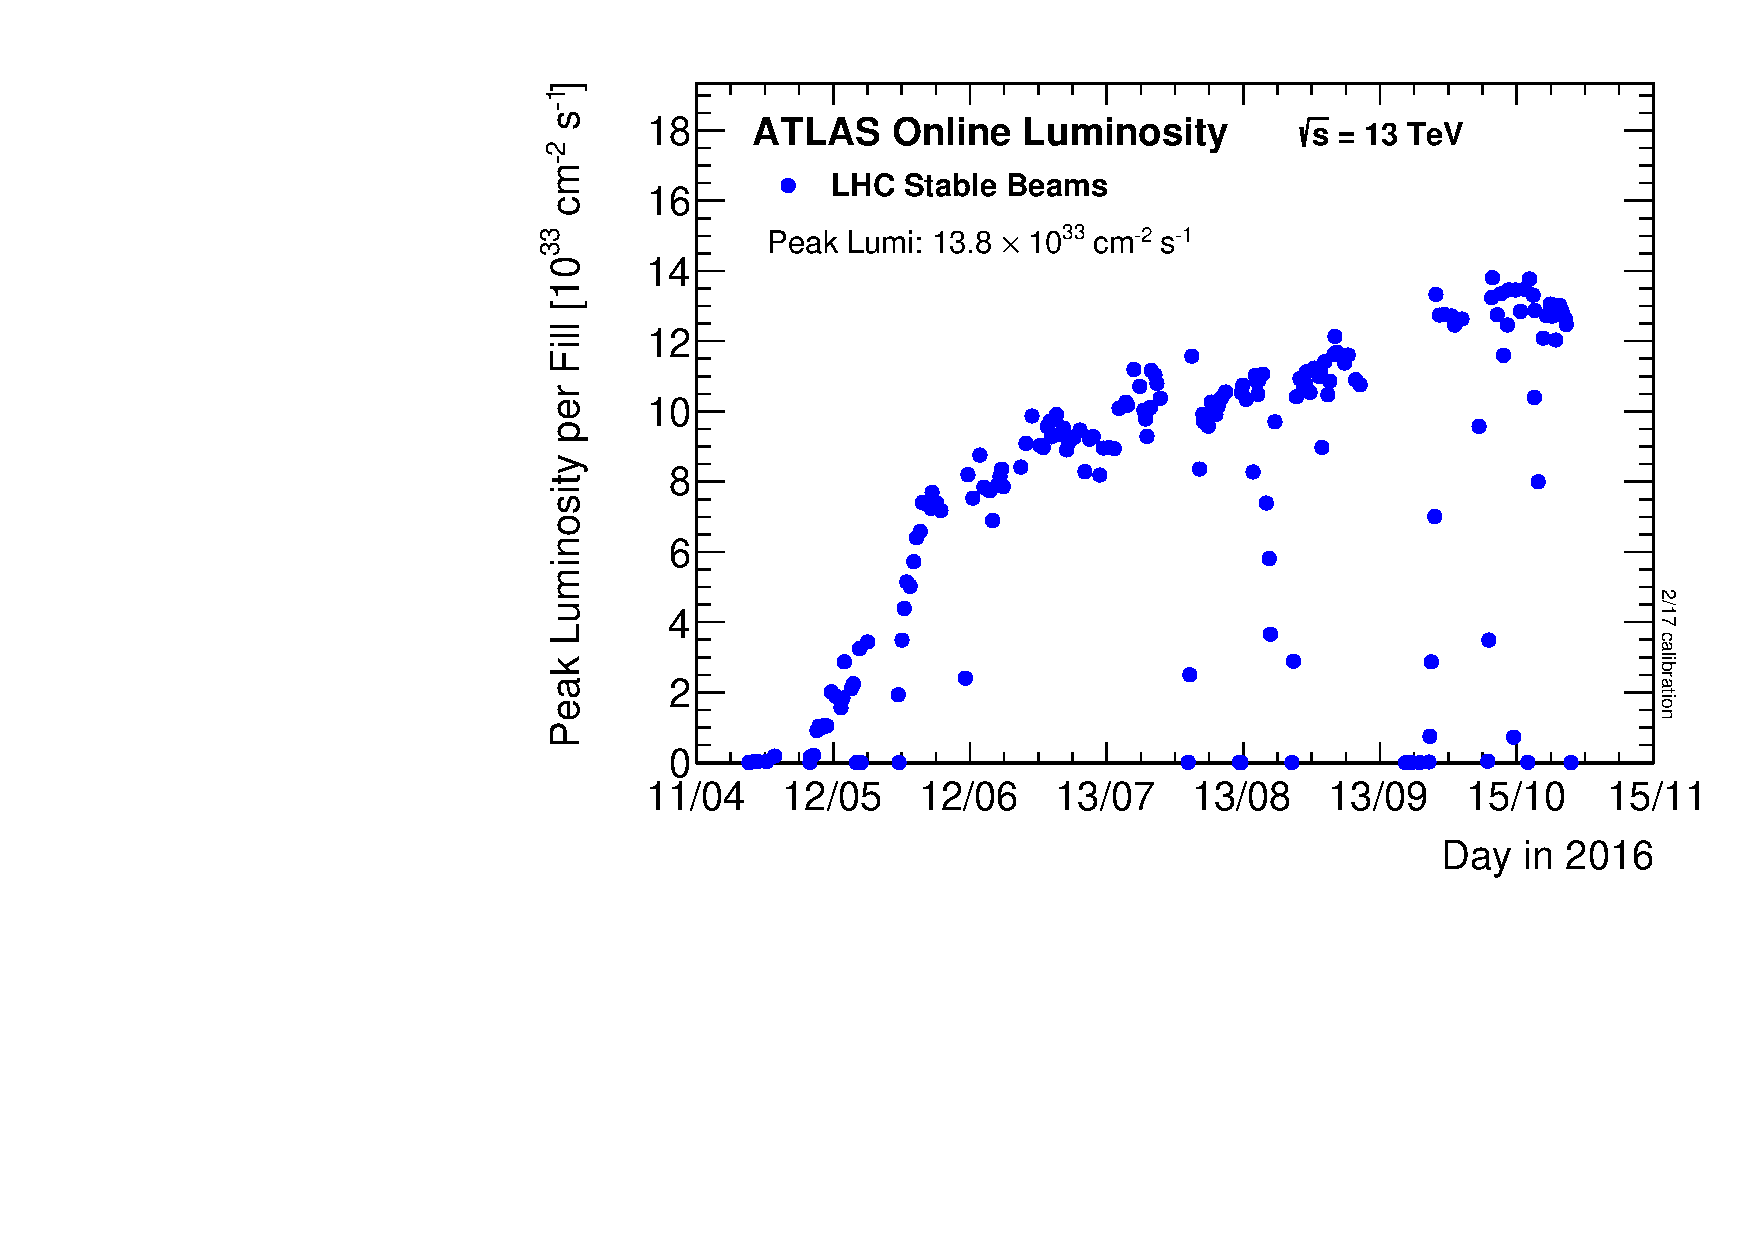
\includegraphics[width=0.95\textwidth]{peakLumiByFill}
\subcaption{}
\label{fig:exp.lhc.peakLumiByFill}
\end{subfigure}
\begin{subfigure}[t]{0.48\textwidth}
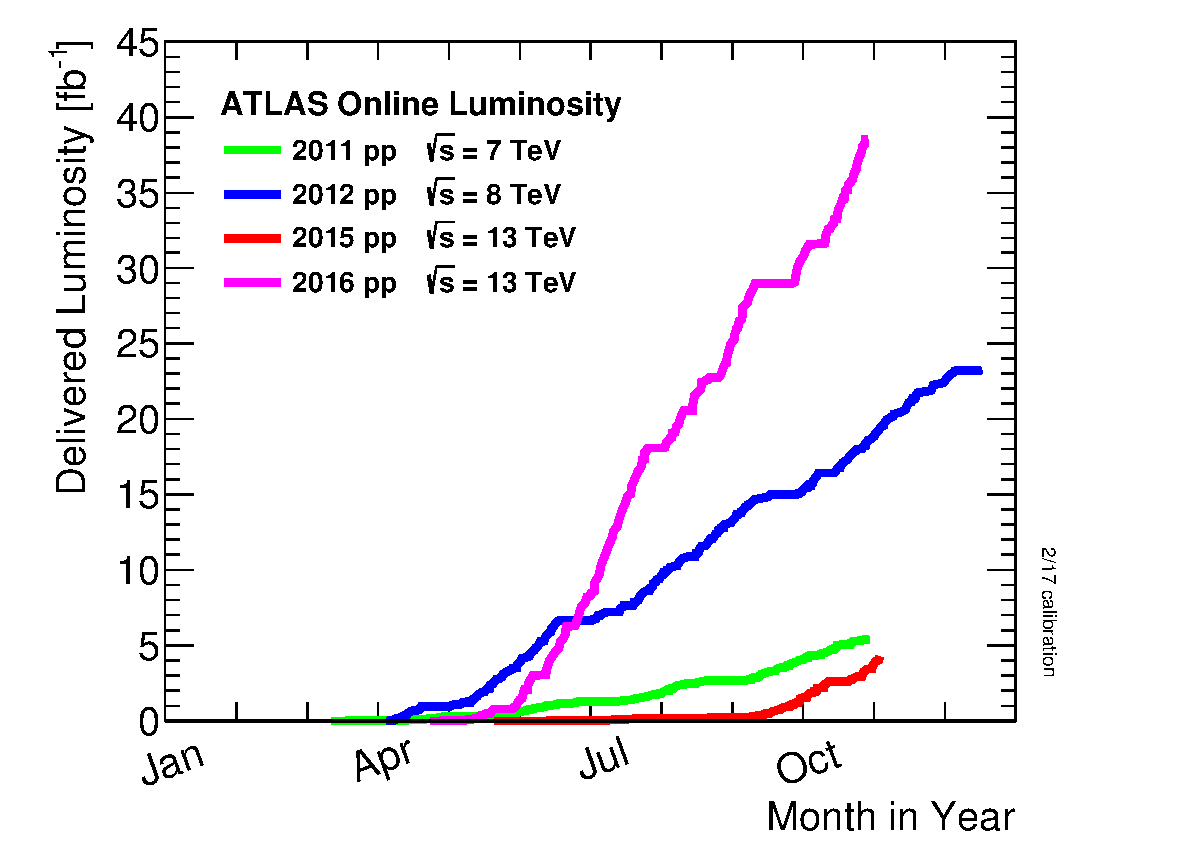
\includegraphics[width=0.95\textwidth]{intlumivsyear}
\subcaption{}
\label{fig:exp.lhc.intlumivsyear}
\end{subfigure}
\vspace{-0.25cm}
\caption{(a) The peak instantaneous luminosity delivered to ATLAS in 2016
and (b) the cumulative luminosity delivered to ATLAS between 2011 and 2016, 
during stable beams for $pp$ collisions}
\label{fig:exp.lhc.peak}
\end{figure} 

The other important characteristic of the LHC is that multiple $pp$ interactions occur at every 
bunch crossing.  This quantity is correlated with the instantaneous luminosity as can be seen 
by comparing Figure~\ref{fig:exp.lhc.peakLumiByFill} and Figure~\ref{fig:exp.lhc.peakMuByFill}. Figure~\ref{fig:exp.mu_2015_2016}
shows that the mean number of interactions per bunch crossing was 25 in 2016 with the peak number of interactions 
reaching up to 50. This causes a computational challenge in reconstructing the physics objects coming from 
one interesting interaction.
\begin{figure}[!htb]
\centering
\begin{subfigure}[t]{0.48\textwidth}
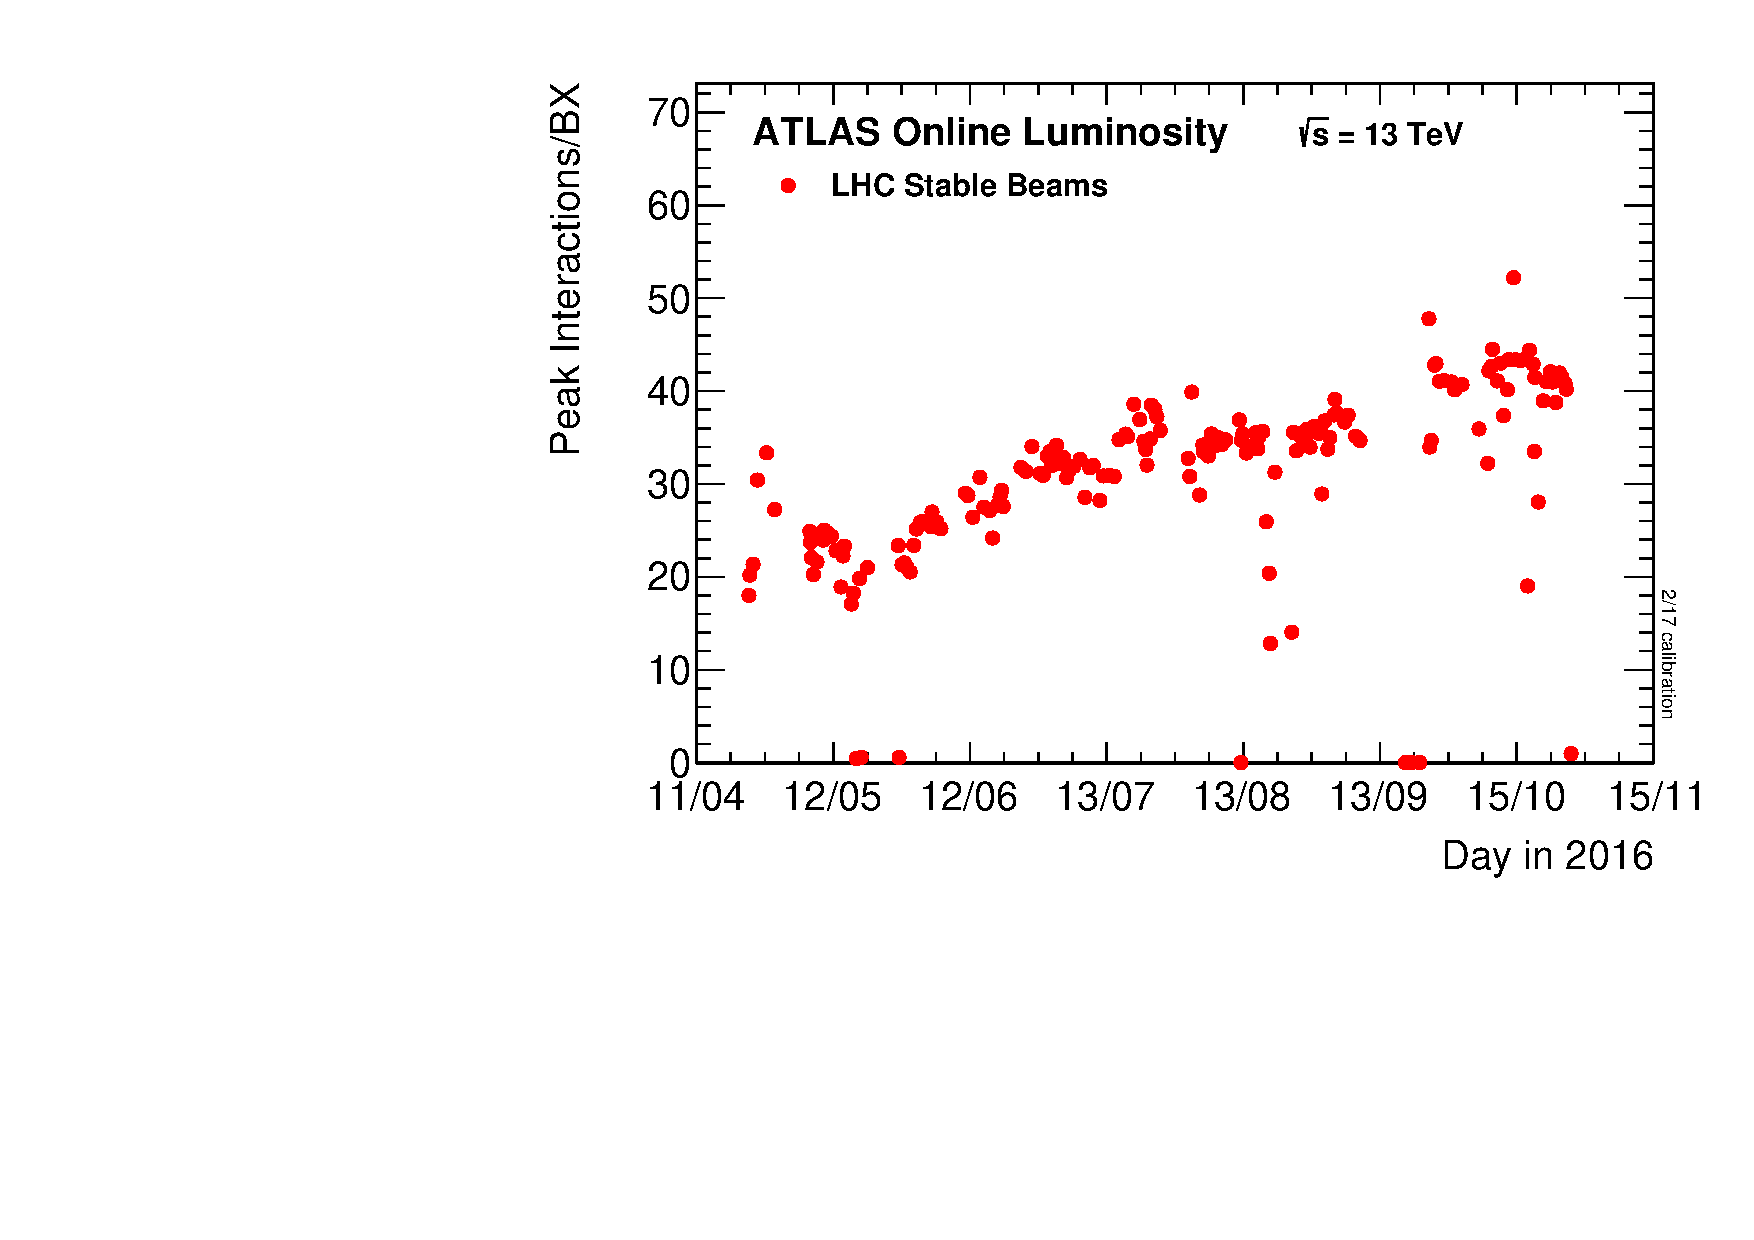
\includegraphics[width=0.95\textwidth]{peakMuByFill}
\subcaption{}
\label{fig:exp.lhc.peakMuByFill}
\end{subfigure}
\begin{subfigure}[t]{0.48\textwidth}
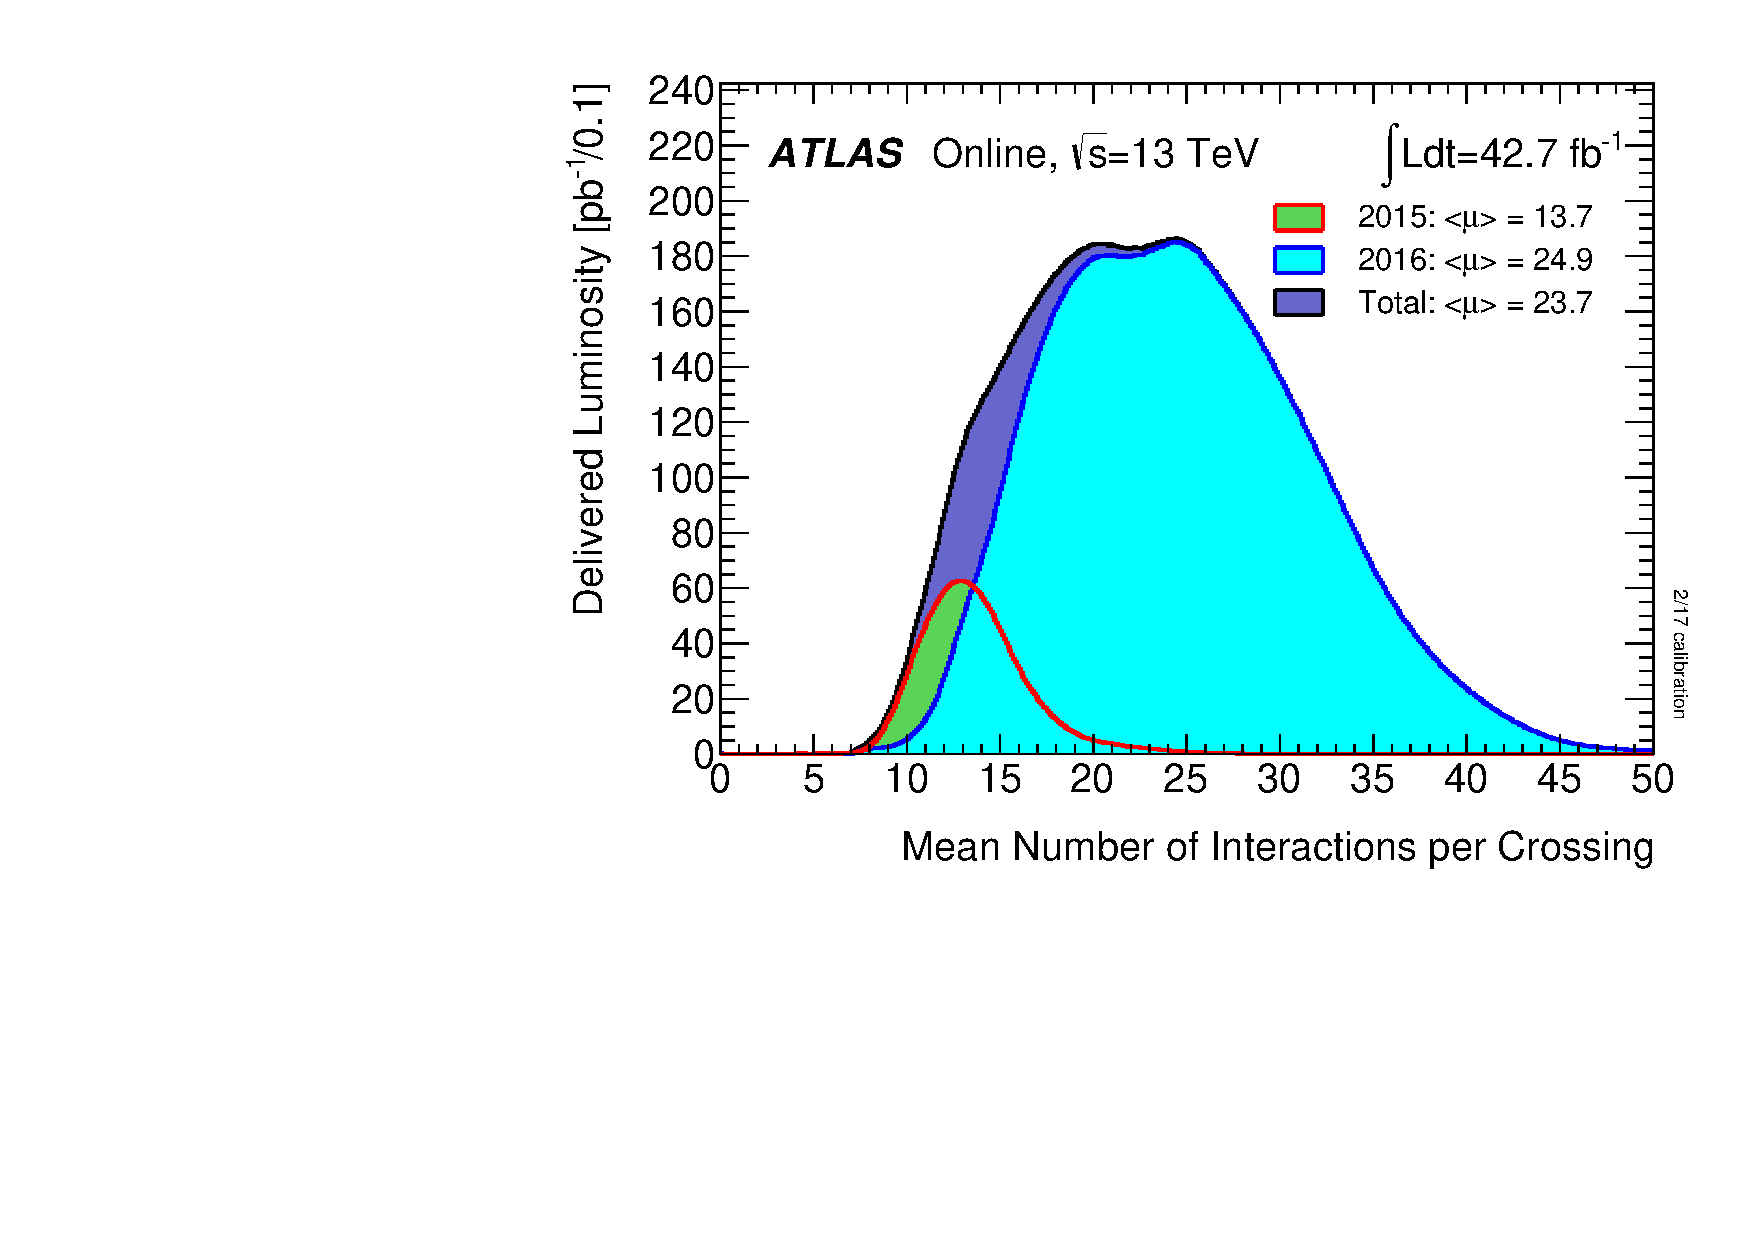
\includegraphics[width=0.95\textwidth]{mu_2015_2016}
\subcaption{}
\label{fig:exp.mu_2015_2016}
\end{subfigure}
\vspace{-0.25cm}
\caption{(a) the peak number of inelastic collisions per beam crossing during 2016 
  and (b) the mean number of these collisions per crossing for 2015 and 2016, during stable beams for $pp$ collisions}
\label{fig:exp.lhc.int}
\end{figure} 
A typical hard scattering of two protons has a large impact parameter leading to low momentum particles in the final 
state. These type of collisions are known as ``minimum bias'' collisions and are considered as background to 
the more spectacular hard scattering that is typical of an interesting event. 
The minimum bias is generally not well understood since it comes from nonperturbative QCD. There are several Monte Carlo generators, such as {\sc PYTHIA} and
{\sc HERWIG}, that are used to estimate these processes by tunning them to 
data.


